%%%%%%%%%%%%%%%%%%%%%%%%%%%%%%%%%%%%%%%%%%%%%%%
%
% Template per Elaborato di Laurea
% DISI - Dipartimento di Ingegneria e Scienza dell’Informazione
%
% update 2015-09-10
%
% Per la generazione corretta del 
% pdflatex nome_file.tex
% bibtex nome_file.aux
% pdflatex nome_file.tex
% pdflatex nome_file.tex
%
%%%%%%%%%%%%%%%%%%%%%%%%%%%%%%%%%%%%%%%%%%%%%%%
\documentclass[epsfig,a4paper,11pt,titlepage,twoside,openany]{book}
%\usepackage[utf8]{inputenc}
\usepackage{csquotes}
\usepackage[italian, english]{babel}
\usepackage{lipsum} %genera testo fittizio
\usepackage{url} %per scrivere gli URL
\usepackage[backend=bibtex]{biblatex}
\usepackage{plain}
\usepackage{epsfig}%Per il logo in formato eps
%Per layout e dimensioni
\usepackage[paperheight=29.7cm,paperwidth=21cm,outer=2.5cm,inner=2.5cm,top=2cm,bottom=2cm]{geometry}
\usepackage{plain}
\usepackage{setspace}
\usepackage{titlesec}
\counterwithout{footnote}{chapter}

%%%%%%%%%%%%%%
% supporto lettere accentate
%
\usepackage[latin1]{inputenc} % per Windows;
%\usepackage[utf8x]{inputenc} % per Linux (richiede il pacchetto unicode);
%\usepackage[applemac]{inputenc} % per Mac.

\singlespacing

\usepackage[english]{babel}
\usepackage{chngcntr}
\counterwithout{footnote}{chapter}

\newcommand\MyBox[2]{
    \fbox{\lower0.75cm
        \vbox to 1.7cm{\vfil
            \hbox to 1.7cm{\hfil\parbox{1.4cm}{\centerline{#1}}\hfil}
            \vfil}
    }
}
\newcommand*\NewPage{\newpage\null\thispagestyle{empty}\newpage}


\addbibresource{biblio.bib}

\begin{document}
\raggedbottom
\widowpenalty10000

%Nessuna intestazione e pie pagina con numero al centro
\pagestyle{plain}


%No numerazione
\pagenumbering{gobble}
\begin{center}
    \begin{figure}[h!]
        \centerline{
\psfig{file=marchio_unitrento_colore_it_202002.eps,width=0.6\textwidth}}
    \end{figure}
    
    \vspace{2 cm}
    
    \LARGE{Department of Information Engineering and Computer Science}
    
    \vspace{1 cm}
    \Large{Bachelor's degree in\\
        Computer Science
    }
    
    \vspace{2 cm}
    \Large\textsc{Final Dissertation\\}
    \vspace{1 cm}
    \Huge\textsc{TODO}
    
    \vspace{2 cm}
    \def\arraystretch{0.7}
    \begin{tabular*}{\textwidth}{c @{\extracolsep{\fill}} c }
    \Large{Supervisor} & \Large{Student} \\
    \Large{Alberto Montresor} & \Large{Stefano Perenzoni}\\
    \Large{Co-Supervisors} & \\
    \Large{Daniele Miorandi} & \\
    \Large{Carlo Caprini} & \\
    \end{tabular*}
    \def\arraystretch{1.0}
    \vspace{2 cm}
    
    \Large{Academic year 2019/2020}
    
\end{center}
\clearpage
\newpage


%Inizio numerazione
\mainmatter
\tableofcontents
\clearpage
\NewPage

\chapter*{Abstract}
\addcontentsline{toc}{chapter}{Abstract}
The recent rise of social media inside the life of our society caused a sharp increment of data availability at the user's level.
Almost everyone relies daily on this type of platform to share their experiences, their thoughts, to interact with friends, to stay up to date with the latest news and also to find new career opportunities.
All these activities carried out by a user leave publicly accessible a great amount of relevant information. The frequency a person logs into a social, the way he or she interacts, the network created by her connections
allow extracting several personal aspects of the single individual. These characteristics can include personality traits, habits and particular attitudes. So, if identified, they can provide a huge business advantage in terms of knowledge of your own customers.

Social media result perfect for this type of analysis because people feel free to post whatever and whenever they want, often giving a strong personal opinion which reveals the behavioural aspects introduced before.
Moreover, these services has been growing exponentially in the number of active users in the last decade. For example, the last \emph{Digital 2020 Report}, carried out by \textit{wearesocial.com}, shows that worldwide there are more than 3.8 billion social media users\footnote{\url{https://wearesocial.com}}.

Even though the current literature has been covering the extraction of behaviours from social media, the majority of studies do not focus on the application of the result in order to get a marketing advantage.
Therefore, there is no software system able to identify, and then let companies use, this information.
For example, none of the research observed took into consideration users' rights in terms of privacy and data protection. 
However, since regulations such as the GDPR are becoming mandatory all around the world, compliance to their rules should not be neglected.
Therefore, the final goal of this thesis is the development of a system for the extraction of personal habits and attitudes from social media that are immediately relevant and usable by a company's marketeers.
This project has been realized at U-Hopper, a small enterprise located in Trento specialized in big data analytics solutions.

The proposed system follows the whole process, from the download of raw data from social media to the conclusive behavioural insights. 
Each phase was developed taking into consideration different aspects. In particular, with respect to the state of the art, this solution follows the main requirements of the GDPR regarding the authorization to access personal data and then the correct treatment of the same.
The prototype is designed to interact with many social networks using their public API to download user's content. The part of insight generation is realized applying many different techniques.
It uses both machine learning models for the extraction of personality traits of the MBTI personality model and non-machine learning algorithm for the computation of better-defined parameters, such as the language used or the periods of activities through the day.
All these algorithms rely on information obtained through different analyses on the downloaded social profiles. For example, the natural language processing of the activities' text represents an important component, especially for the identification of the personality characteristics.
The system was then developed as a web service accessible and exploitable thanks to a series of well-defined endpoints.

Finally, a web dashboard was realized to help the evaluation of the system. Thanks to some architectural choices made, it also allows to observe how the identified insights varied over time.
This dashboard was then used to analyse and observe more than twenty different profiles.
\clearpage
\newpage

\chapter{Introduction}
\label{cha:introduction}

During my internship at U-Hopper, I had the opportunity to develop this Thesis as a result of my experience inside the company. 
\textit{ U-Hopper is a research-intensive deep-tech SME, headquartered in Trento, providing big data-enabled solutions and technologies for the government, retail and manufacturing sectors. U-Hopper has received numerous awards for its innovative solutions, including, among the others, the Lamarck prize (2013), a EC Seal of Excellence (2015), the Innov@Retail prize (2016) and a nomination for the 2017 EC Innovation Radar Awards.}.
The company is active in many different domains such as retail and tourism and offers a variety of competences including chatbots, analytics, and machine learning.
Thanks to Tapoi\footnote{\url{www.tapoi.me}}, an innovative data intelligence solution, U-Hopper is also into the sector of user profiling.
It allows businesses to deliver personalized experiences to their customers through the mining and analysis of their activities on social networks.
Thus, the extraction of behavioural insights can be a valuable aspect since being aware of how an individual comes to a decision helps to provide each customer with the right tailored content.


\section{Motivation and business requirements}
Dissatisfied customers represent a dangerous threat for companies and their brands. Thus, it is fundamental for a business to track audience satisfaction and do whatever it can to fulfil their want.
Dissatisfaction can impact a company in two different ways. 
First, those who are not completely satisfied would behave passively towards the business, reducing the number of purchases, and therefore stop being consumers of its products and services.
Moreover, those who are more active and extroverted could interact with others and convey their disappointment.
Overall, a large number of unhappy customers will entail a significant loss of customers.

This problem is of particular interest to those typologies of companies that follow a \emph{business-to-customer (B2C)} sales process,
with a wide customer base and which interactions with their audience are characterized by online relationships.
This relation can be purely telematic, as in the case of e-commerce, or it can support a physical one where the material interaction is unavoidable, as in the case of banking and insurance sectors.

For this kind of businesses, customers' satisfaction is not trivial to accomplish since each one of them has different needs and requests and standard methodologies do not adapt well for everyone.
Thus, over the past few years, personalization of customer experience has become vital in order to inspire an honest and natural emotional response.
It is then important to be able to access information which allows marketeers to offer fully tailored contents, through a specific mean of communication and with personalized messages to meet each individual's requirements.

While, thanks to Customer Relationship Management (CRM), data related to the direct interaction between customer and company has already been deeply explored, social media networks gave access to more personal information allowing a deeper understanding of the person.
The system discussed in this thesis proposes a solution that goes further than the diffused purchase history-based personalization.
It aims to provide companies with the ability to extract readable and valuable insights about singular individuals from their activities online.
The final goal is to make available actionable insights about users' behaviour, demographics and attitudes.
In particular, this dissertation focusses on the extraction of personality traits to obtain a detailed description of a person's behaviour and reaction to a number of observed solicitations



\section{Customer insights}
\textbf{General introduction to customer insights, different types, benefit for businesses}

\textbf{At the end, a short focus on psychometrics}

\section{Extraction of personality models}
According to neuroscientists Adelstein et al., personality describes human behavioural responses to wide classes of external stimuli \cite{adelstein2011personality}. It works as an adaptive system for taking in, organizing information and driving the response to inner and outside demands \cite{block2002personality}.
The parameters of the adaptive system represent the variation of the same from person to person and, therefore, characterize uniquely every individual. These parameters are also referred to as personality traits in several different personality models studied over the years.
Each model includes its range of traits which combinations describe several personality types.
Researchers have shown clear connections between general personality traits and many types of behaviour.


Some fundamental traits describe the type of relationship a person has with the outside world and the way he or she communicates \cite{lima2016predicting}.
Thus, to facilitate communication, recently, businesses are using personality models to gain a better understanding of what drives the interests of a person.
This approach is showing clear benefits in many different applications.
In the field of Human-Computer Interaction, users prefer interfaces designed to represent personalities that most closely matched their own \cite{nass2000does}.
Some studies have also suggested connections between customer personality and marketing. Through techniques more focused on the target audience, it is possible to profile individuals, and tailor advertisement automatically displayed based on their personality \cite{bachrach2012personality}.
Therefore, the ability to identify people's personality or, even better, details of their personality traits through well-defined models is a significant competitive advantage since
we would have a precise representation of the customer's reasoning process.

%Big5
\subsection{Big Five personal traits}
While several models exist, the \textit{Big Five}, also known as the \textit{five-factor model} and the \textit{OCEAN model} is one of the most well-researched and widely accepted taxonomies among scientists \cite{mccrae1992introduction, mccrae1987validation}.
It formalizes personality along 5 domains, namely Openness, Conscientiousness, Extroversion, Agreeableness, and Neuroticism. Each one of these traits is continuous and usually ranges on a scale from 1 to 5.
High openness marks imagination, creativity, and curiosity in learning and exploring new things. Conscientiousness represents self-discipline and attention to details.
Extroversion measures preferences for interacting with other people. Agreeableness reflects the extent to which a person is generous, trustworthy and always willing to help others.
Finally, a high score on neuroticism indicates a tendency to get stuck in negative emotions.
At the two extremes of each trait, two separate aspects reflect a particular behaviour. 
For example, conscientiousness is bounded by carelessly at the lowest end and by organization and efficiency at the greatest one.

Since its first definition, this model rapidly became one of the standards in the psychological community, largely accepted by the most share of scientists since it allows to describe accurately the traits of a singular.
However, concerning the exploitation of personality information in the work and marketing environments, it received some critics about the extraction of actionable insights\cite{hough2003use, patton2014career}.
Indeed, since each trait is represented by a real number between 2 extremes, it has been argued to be hardly readable and therefore less valuable for fields such as marketing and business.
Thus, structures based on clearer distinctions are often preferred.

%MBTI
\subsection{Myers-Briggs Type Indicator}
\textit{The Myers-Briggs model}, also called \textit{Myers-Briggs Type Indicator, or MBTI}, is the most common alternative to the Big-Five model.
Contrarily to the former, there are discussion about the MBTI and its limitations in reflecting the whole personality system. 
Boyle and Barbuto are two of the scientists that presented a number of psychometric limitations pertaining to the validity and reliability of this model \cite{boyle1995myers,barbuto1997critique}.
However, many of their arguments have been proved wrong by Furnham who demonstrated several correlations between the dimensions defined by Myers and the big five factors \cite{furnham1996big}.

The MBTI is a categorical model, based on the conceptual theory of Jung and developed by Katharine Briggs and Isabel Myers who used four different dichotomies to evaluate the personality of people \cite{jung1971personality}. 
A first one differentiates a person's attitude in either extraversion (E) or introversion (I).These two preferences describe if one focusses on external stimuli, such as action and interaction with other people or internal ones like self-reflection.
Two perceiving functions, sensation (S) and intuition (N) describe the process of gathering new information. On the one hand, people who trust tangible and concrete facts; on the other hand, those who tend to find patterns and meaning also regarding future possibilities.
The third cognitive function is that of decision-making which can be thinking (T) or feeling (F). While thinkers make reasonable and consistent choices and reflect over consequences applying a rigid set of rules, feelers tend to emphasize with the situation considering the needs of people involved
Finally, there is the lifestyle preference function dichotomy, judging (J) or perceiving (P). Judging types like the outside world to be structured; according to Myers, they prefer to ``have maters settled''. On the contrary, perceiving personalities like it flexible and spontaneous and tend to ``keep decisions open'' \cite{myers2010gifts}.
There are 16 different types of personality given by the combination of these 4 cognitive functions identified by 4-characters codes such as ``INFJ'' or ``ENFP''.

%ML Problem
Using a categorical model, the extraction of personality from social media activities is a \textit{machine learning} problem, precisely, it consists of numerous classification tasks, one for each of the four variables.
Machine learning is one of the most talked-about fields of computer science and many sources give their own definition. Basically, ML deals with allowing a computer system to ``learn with data, without being explicitly programmed" \cite{samuel1959some}.
It has been applied in many contexts, such as decision making, optimization problems, forecasts, and predictions.
Nowadays, we face ourselves with machine learning in everyday life: home assistants, security surveillance, music and shopping suggestions, customer services are strongly powered by artificial intelligence.
These services rely on data to learn how to work as good as possible: they are trained with samples of data similar to what they expect to receive by their users: the more accurate, exhaustive and in large quantities they are, the better the system learns. Therefore, data have a very central role in machine learning problems.

A classification task has the goal of assigning a belonging class to a given object. The input is composed by a tuple of \emph{features} that characterize the object, usually made by numbers, and the output is a categorical variable, such as a "yes/no" label. In other words, it can be seen as a mathematical function, that maps a vector $ \boldsymbol{x} \in \mathbb{R}^n $ to an answer $ y \in C $
\begin{gather*}
\begin{split}
f & \colon \mathbb{R}^n \to C \\
f & \colon \boldsymbol{x} \mapsto y
\end{split}
\end{gather*}
where $C$ is a set of possible categories.
For example, in one of the four classifiers for this problem, $ \boldsymbol{x} $ represents a user and her activities on the social media, and $C = \{\text{\texttt{Introvert}, \texttt{Extrovert}}\}$

\section{Research objectives}
Extraction of behavioural insights from social media has recently attracted the attention of both researchers and businesses.
Even though the latter has released a couple of solutions, these fit better for personal and psychological use rather than a commercial one.
The main objective of this thesis is to design and develop a solution that can be used by a company to personalize customer experience with respect to individual abstract preferences.
Therefore, the question it answers is: \textit{is it possible to understand costumers behaviour from their online profiles and activities?}

The designed system should be able to work with numerous social media platforms to have a wide variety of data sources.
Finally, the principal aspect that it must always satisfy is the \emph{ability to use the result}. Indeed, extracted insights need to be actually actionable, directly by the marketing department or in conjunction with further analysis, to represent a competitive advantage.
\section{Outline}

Chapter 2 describes the state of the art. Chapter 3 introduces the design of the solution. It focuses on used components and algorithms, their logic and their interfaces. 
Chapter 4 shows how the mentioned components are implemented and integrated. It follows the implementation of the algorithm and the evaluation of a general prototype of the proposed system. 
Chapter 5 concludes the thesis with some observations and future work proposals.
\clearpage
\newpage



\chapter{State of the Art}
This chapter presents the current state of the art regarding insights extraction on social media.
Many aspects of online users have been explored in order to profile customers.
"Then, there is a focus on what has been done in terms of providing actionable personality insights."

%II
Some studies aimed to identify clear demographic characteristics based on both the analysis of a user's activities and her network inside the social media. 
Twitter is commonly used for the extraction of gender \cite{miller2012gender}, age or age groups \cite{culotta2015predicting}.
Also, a person's family status is inferred through the detection of life events such as the birth of a child and a marriage \cite{dickinson2015identifying}.


%III
The literature also presents many examples of latent attributes extraction.
Some of the most remarkable research has been carried out by the \emph{World Well-Being Project} \footnote{https://wwbp.org/}; a research center which used 
social media to measure attitudes and personal characteristics such as optimism and pessimism \cite{ruan2016finding}, temporal orientation \cite{schwartz2015extracting}.
Many different social networks have been explored as well as many aspects that are not limited only to text but also include images and social interactions.
Finally, it is a common practice inferring behaviour through a variety of personality models.

%IV
However, what has been done is almost completely focused only on the feasibility of extracting attitudes' insights from online activities rather than a commercial use of the obtained information to generate a marketing advantage.
So, the literature presents only a few systems which satisfy the right requirements for an application in the real world, such as those imposed by the GDPR TODO CITE.

\section{Customers Profiling}
A precise and detailed description of social media users requires the analysis of many aspects of social media. 
Indeed, understanding the users means being able to quantify and qualify how they present themselves \cite{schwartz2013personality}.

Many of the systems proposed for social media analysis use as fundamental component features that describe interactions of users, such as the number of followers, mentions, likes, and comments.
%Questa analisi di interaction è stata esplorata molto, partendo da solo numeri statici, all'osservazione dinamica della rete...
This type of analyses has been largely explored since studies about user influence and social engagement. First, raw measures publicly available on social media were used to calculate metrics to represent effectively the user's influence \cite{oviedo2014metric}.
Further research proved that simply observing ground numbers of a profile can lead to a misunderstanding. Cha stated that the indegree alone (number of followers) reveals little and suggested to consider shares and mentions from other users \cite{cha2010measuring}.
D. Romero et al. observed influence analysing the propagation of web links over time using both the structural properties of the network as well as the diffusion behaviour among users \cite{romero2011influence}. They also regarded the \emph{passivity of a user}, a measure of how difficult it is for other users to influence him, and used it to weigh the tweets propagation network. 
%Cambia da social a social a seconda di unilaterale o bilaterale
Many different networks can be explored on social media in order to identify influence, communities, and trend topics applying the myriad of network concepts and analyses such as degree centrality and modularity \cite{chae2015insights}. 
The nature of these graphs can change regarding the platform's characteristics and the aspect we are looking at. Li complained about undirected networks, such as the Facebook friends graph and proposed a method based on the \emph{Share/Reply/Mention} directed network to capture user influence \cite{li2014social}.
These observations are usually used to profile a person's social environment and to assess his or her role inside it. 

%Dopo di che, si ha iniziato a fare analisi del contenuto
%Prima con hashtag e url, poi con altri servizi
A second fundamental point carried out by literature on social media is the analysis of the context the user is talking about.
Obviously, being aware of what topics drive someone's interactions is essential to profile his or her interest. 
Moreover, they can be used to reduce other types of analyses to a specific field of interest. For example, focussing on users' influence in sports discussions.
To understand context, it is necessary to observe the content of the messages which is usually composed by text and images or videos.
Firstly, keywords in the activities were used to identify topics \cite{cha2010measuring}. This methodology shows some clear issues, especially when used for social media when messages tend to be extremely abbreviated through acronyms and slang words.
Other approaches, feasible in a limited number of platforms, proposed to use most used hashtags to obtain linguistic content starting from the activities \cite{pennacchiotti2011machine}.
Finally, a more general technique is using the tree of Wikipedia categories to characterize the user's interests. 
This method fits well with both text and multimedia content thanks to a number of services that apply semantic analysis techniques to extract relevant entities \cite{torrero2018wikipedia}. 

\section{Behavioural insights}
"Psychometric profiling is the process by which your actions are used to infer your personality."

The literature presents many different techniques for the extraction of behavioural information which are all based on the most used personality models to study specific traits of an individual.
The models proposed are classifiers or regression one depending on which personality taxonomy is being applied.
Each model is specialized to a single specific personal characteristic, for example, using the MBTI personality model there are 4 classifiers, one for each cognitive function.
Almost all models presented work on social user composed by the totality, or a portion, of their timeline rather than single activities since linguistic information contained by a single short activity is not enough to accurately predict personality aspects \cite{mairesse2007using}.

The feature extraction shares some fundamental aspects in the majority of systems. The results of the analysis seen before represent two essential groups.
Indeed, understanding a user's network helps understand how he or she reacts to external stimuli. Therefore, it plays a crucial role in the extraction of behavioural insights from online activities.
Also, research has shown a strong correlation between discussed topics and personality aspects of a person \cite{kern2016gaining}.
Guntuku et al. proved that studying semantic concepts contained in posted images can give a significant performance gain in predicting personality traits with respect to the \emph{Big Five model} \cite{guntuku2017studying}.
However, the literature contains a very few number of proposals that considered the content of the activity and are usually confined to hashtags and key words in the text \cite{ruan2016finding}. 

Regarding features that describe the social presence of a person. These are usually included by the majority of models. Although some are limited to basic information such as the number of followers, following or friends, the number of activities, and their frequency \cite{quercia2011our}.
Over time, the literature presented the application of more complex features, obtained as results from further analysis of the user's network such as interaction patterns by a person towards the author of the post \cite{dickinson2015identifying}.
For example, significative patterns could be a high retweet ratio by users who do not retweet much other sources by or an elevate number of interactions by users with many followers. However, these last observations need the permission of each person belonging to the analysed network to be respectful of GDPR requirements. Thus, even though they could give great results, their lawful application in the market is quite intricate.

Then, there is a third fundamental group of features which is probably the most important one.
Since psychological studies proved that there is an effective relationship between linguistic style and personality aspects, understanding detailly how an individual writes is a crucial step \cite{pennebaker1999linguistic}.  
Some of the most common and basic features are word counts, sentences per activity, word per sentence, and punctuation count. These have been applied by the majority of models with great results in many different environments.
For example, Farnadi recognized personality of YouTube vloggers using the script of their videos to extract this linguistic information \cite{farnadi2014multivariate}.
Furthermore, more recent studies have tested features from specialized and complex tools for text analysis. These can reveal precisely thoughts, feelings, and motivations of the text's author.
The \emph{Linguistic Inquire and Word Count (LIWC)} developed by Tausczik and Pennebaker is certainly the most used one \cite{tausczik2010psychological}.
Other services that have been tested are the \emph{MRC Psycholinguistic Database} and the \emph{NLPRO}, developed by oNLPLAB \cite{wilson1988mrc, tsarfaty2018natural}. Lima et al. tested the three of them concluding with the first one as the most performing one \cite{lima2019tecla}

Far vedere diversi tipi di analisi fatti per la personalità
Poi dire che molti si basano sul big5 e far vedere quelli sull'MBTI
\section{Commercial applications}
\clearpage
\newpage

\chapter{Design and methodology}
This chapter presents the architecture of the system. Starting with a basic schematic view, it is showed what fundamental components compose it, their role, how they work and how they communicate each other.
%Then description of specific choiches
Then, the architecture is detailed more. Each step, starting with the download of raw activities and ending with the final user's attitudes, is described specifying what choices have been done and why.

At a high level, the system takes as input an ID representing a user in the system.
This user is associated with many IDs, one for each social network he or she is registered in and has provided access to.
These are used to download her profiles which, together with their respective activities, are used to classify the user's behavioural aspects included in the analysis.

\section{Requirements}
The main functional requirement is that the system has to be able to extract a set of behavioural aspect that characterise the user taken as input.
All the social network the user has registered must be analysed for both the social profile and the activities.
The architecture should allow the addition of new users into the system and the removal of existing ones. Then, once a system user is created, it must be possible to register and remove new social media account.
During the download of new activities, the system should let use a filter or a counter to exclude unnecessary activities.
Finally, the set of attitudes that can be classified must be defined a priori. For example, it can be equal, but not limited, to the 4 cognitive functions of the MBTI previously introduced.

\section{Process logic}
Here, the fundamental process followed by the system is introduced.
Each step covers a section of the process required to go from the simple user ID to the final insights that the system aims to provide.
The whole flow is sequential. Each activity takes as input the output of the previous one
There are 4 essential steps which can not be excluded despite specific design choices:
\begin{enumerate}
    \item Download profiles and activities from social networks.
    \item Analyse the downloaded data to extract significant features.
    \item Classify the profiles.
    \item Put together the partial results from each classifier to generate the complete user image.
\end{enumerate}
The steps are executed the same number of times and each one immediately follows the previous one with the requirement that the former must have ended for the latter to start.
The only exception can be found for the first two activities which could be grouped together. Indeed, once an activity is downloaded this could be immediately sent to the following action while a new one is put on download.
However, before the classification could be performed the whole profiles should be completely downloaded and analysed.
Finally, the final result can be stored. So, all the process is coordinated by a single call which start with the download phase and end the annotated user.

%This steps describe abstractally the flow followed by the system
%These functionalities are later in different components which purpose is to follow this process.
These steps give a general description of all the jobs required to go from the raw user identifier to its classification.
These functionalities are subsequently realized thanks to different components with the purpose of following this abstract process.
The final components of the system may vary according to the architectural choices made.

\section{Classificator's architecture}
While the first two steps are quite common and do not present significant choices that could modify the system, the third one deserve to be observed in more detail.
In the extraction of insights at user level, it is essential to understand precisely how the social user is defined and by what data it is characterised.
The state of the art rarely took into consideration different approaches. Usually, all the information obtainable by the totality of the activities downloaded are put together to represent the user ready to be classified.
It means that, at each request, all the downloaded activities are merged into a single user that summarise what has been provided by the social media.
At first, a solution of this type might work if the goal is to verify the feasibility of a specific classification in order to be able to measure its performance quickly and easily.
On the other hand, when it comes to the production environment, this technique presents some evident lacks that need to be considered.
For example, one main issue concerns TODO %The integration of the result once new activities are posted. We don't want to recompute entirely the profile

Starting from this last problem I worked on three different alternatives. These three proposals are the feasible solutions that answered to a series of questions and critical points that emerged during this design process. 
\begin{itemize}
    \item Architecture \textbf{per aggregation}: the classification is performed on the so-called user aggregates. User aggregates represent the totality of the feature extracted by the profile and its activities. In the moment new activities are downloaded from the social profile, the previous aggregates are updated and then stored ready for the classifications.
    \item Architecture \textbf{per activities}: each activity is classified singularly. Instead of the features, the result of each activity is stored and then put together to generate the insight at a user-level.
    \item Architecture \textbf{per batch}: the classification is performed on the aggregates obtained from a batch of activities. Batches are disjoint sets of downloaded activities. Each is classified independently and its result is stored. These partial results of a specific user are merged together to get the final result. 
\end{itemize}

I evaluated and compared these three alternatives against six criteria considered fundamental with respect to the initial research question.
The six bases are: computation complexity, result's accuracy, GDPR compliance, result's flexibility, storing, and scalability.

\subsection{Computation Complexity}
The performance of each propose strictly depends on the trade-off between a single classification and the aggregation of features from many activities.
Assume that the cost of a single classification is equal to the number of features M, $\Theta(M)$.
Estimate now, for each solution, the computational complexity of the download of N activities and the user's classification.
Firstly, It must be noticed that the first two steps of the process, the activities download and their analysis, are not affected by the architectural choice. Therefore, to keep everything clearer, their contribution will be omitted from the following estimations.

Assuming that the aggregation algorithm just iterate on each post of the timeline a single time observing each one of the M extracted features. So, its computational cost is $\Theta(N*M)$.
As already said, Using user's aggregates implies to compute the classification on its totality at every request to the system. So, this method's complexity considers the number R of requests which is obviously constantly growing. 
It can be formalized as \textbf{$\Theta(N*M) + \Theta(M*R)$}.

Regarding the second alternative, while it is no longer necessary to aggregate the analysis of each activity, it is required to merge together each singular result in order to obtain the final insight.
Moreover, the classification is performed N times on the exact number M of features.
So, the complexity of the solution activity-based is \textbf{$\Theta(N*M) + \Theta(N)$}.

To analyse the last solution, the batch-based one, it is not necessary to define how batches are composed in detail.
The N downloaded activities are somehow partitioned into B batches with $B \leq N$.
Each batch's content is aggregated with the same algorithm introduced before. In general, it is not important how many batches there are, the aggregator will still work on M features of the N activities.
Finally, the B batches are classified singularly and their results are then joined together.
So, the complexity is \textbf{$\Theta(N*M) + \Theta(B*M) + \Theta(B)$}.

To conclude, since the architecture aggregation-based considers in its formula the number of request to the system, it is not scalable in terms of increasing loads.
On the other hand, the other two alternatives are computationally similar. The differences between the two stay in the number of classifications done and the final aggregation of partial results.

\subsection{Accuracy of the result}
Regarding the final result obtained by each of these three methods, even though it would be better to carry out a detailed evaluation process, some general observations can be done without any implementation test.

Starting with the architecture per batch, user aggregates are easy to calculate since they generally consist in the sum of many values or in their average. Thus, they are precise and represent correctly the user's values.
However, even though until now I have been talked only about features extracted by the online activities of the user, other useful information is represented by that related to the social profile. For example, fields such as the number of followers, that of people followed, the user's location, and many other help describing the individual, her social presence and connections.
In this case, at every download request, this information contained in the user aggregate is updated with the new one. Consequently, the snapshot of the old status is lost.
This means that the activities are not associated with the exact moment they were written but they all treated the same way without differentiating the social situation of the user.

This last issue is partially solved by the activity-based methodology because in the features used to classify each activity can be included that information about the social user.
However, this data is taken in the moment the social network's API are consulted so it is not perfectly accurate for each post but it can represent a good approximation.
On the other hand, this alternative involves two major obstacles. Firstly, it has been proved that, especially in the case of psychological studies, text represent the first source of information. Typically, on the social media users tend to write short posts composed by just a pair of sentences. 
Thus, what has been argued is that the quantity and the quality of the extracted features do not allow a precise classification of behavioural aspects.
Secondly, once every single activity is classified, they must be merged together to generate the user's insight.
In the case of categorical results it is not clear how singular results should be merged and how each one should be weighted with respect to the others.

Finally, the architecture per batch has the same advantage of the one per activities because each batch would be characterised by the features that describe the social status of the user.
So, each batch of activities, depending on when its was downloaded, includes some data describing that information mentioned before.
Moreover, the problems of the previous technique here are less pronounced. Indeed, batches can include the right number of activities in order to get the right amount of features.
Also, during the aggregation of partial results, each one could be weighted both dimensionally and temporally giving so more freedom to adapt the implementation.


\subsection{GDPR Compliance}
Design a system that respect the last regulations about the protection of personal data is one of the goals of this thesis.
In this design phase, some requisites from the GDPR emerged as crucial aspects. In this chapter it is explained how the three different architectures satisfy or not the requisite of data minimisation and that of data accuracy already introduces in chapter 2 "State of the Art".

Starting as always from the solution per aggregation, it implies to store the user aggregates so that they can be updated or classified whenever the user wants.
Even though this data is composed by the relative features extracted from the activities and not by the activities themselves, they still contain personal and sensitive that need to be protected.
Then, as discussed is the previous section, info about the social status are unique and dated to the last upload so they are less accurate with respect to the whole timeline.

Using one of the other two alternatives, the situation changes markedly because they do not require to store the activities nor the extracted features. It is enough to memorise all the partial results and some descriptive information, such as the number of activities and their date, in order to be able to join them together.
The solution activities-based, compared to the last one, brings more profit with respect to the accuracy issue. Indeed, it gives the opportunity to complement every single activity with the social status in the moment it was posted while batches still implies a minimum approximation.

\subsection{Flexibility of the result}
This small chapter gives a focus on the benefits regarding the result's flexibility rather than criteria that need to be met.
Depending on this architectural choice the system could allow the composition of the final results with different options. For example, by taking into consideration only a subset of the whole user's timeline

Using the user aggregates, it is quite difficult to act on the final result once it has been classified.
Indeed, the result is the direct output of the subset of aggregates the classification algorithm uses. So, the only way to affect the result is by working on these aggregates which include the whole timeline and are unique for each user.
%Quindi l'unico modo per "filtrare" l'input del clasificatore sarebbe quello di riscaricare ed analizzare nuovamente solo le attività che rispettano il filtro desiderato

The architecture activities-based is for sure the one with the highest flexibility. Indeed, it is immediate excluding some activities that do not meet a specific requirement.
For example, it would be possible to compute the user only for her social presence during the summer periods or during the weekends. 
So, memorising a flag together with the result would be enough to subsequently filter the final result.
These flags are not limited only to datetime aspects. For instance, they can be used to differentiate posts that talk about sports from those that talk about politics.

With the solution based on batches, it becomes possible to treat each batch differently. It all depends on how the batches are composed.
For example, batches that cover specific time periods give the opportunity to observe temporal variations. Then, they could be filtered depending on a exact term.
Also, each batch can be normalized regarding the number of activities it contains in order to weigh its contribute on the final result.


\subsection{Storing}
Here is briefly discussed where, in the system, data persistence needs to be implemented
Then, it is observed how the data model affects the system and, in particular, its evolution.

To compute the user aggregates, persistence must be implemented on the component that perform the aggreagation so that they can be updated at every new download.
Then, the results of the classifications need to be stored. Also, the activities collector should know which is the last activity downloaded for each user in order to not count them multiple times.
The features the system memorise are always known a priori depending on what classifications the system performs. Consequently, the removal or the addition of some features, for example to improve or add a new model, involve adapting the whole data model and the download of the whole user's timeline.

For the other two proposals, it is necessary to have data persistence on the component that deals with the classifications so that the result of each batch or activities can be stored.
Obviously, the activities collector always need to know which is the last downloaded post.
It is quite immediate to add new services at the system since the features extracted do not need to be memorised but are immediately used from the next component. So, the data model is affected only on the result aspect in the case new classifications are added.

\subsection{Scalability}
This last aspect does not vary much from one solution to another. All three architectures allow the parallelization of the independent classifiers.
In addition, for the two architectures based on multiple classifications, these can be parallelized since both each batch and each activity are independent of the others.

%Capitolo nuovo

\section{Components's logic and interaction}
After this analysis, it was decided to focus on the third proposal, the batch-based architecture.
The one based on the user aggregates is quite basic has several shortcomings in many of the observed aspects.
The other two share many advantages but regarding the accuracy of the result, the activity-based solution has some complications not included on the other one.
However, as said before, that aspect was analysed through general observations and testing both the architecture would give a more detailed overview.

\begin{figure}[htp]
    \centering
    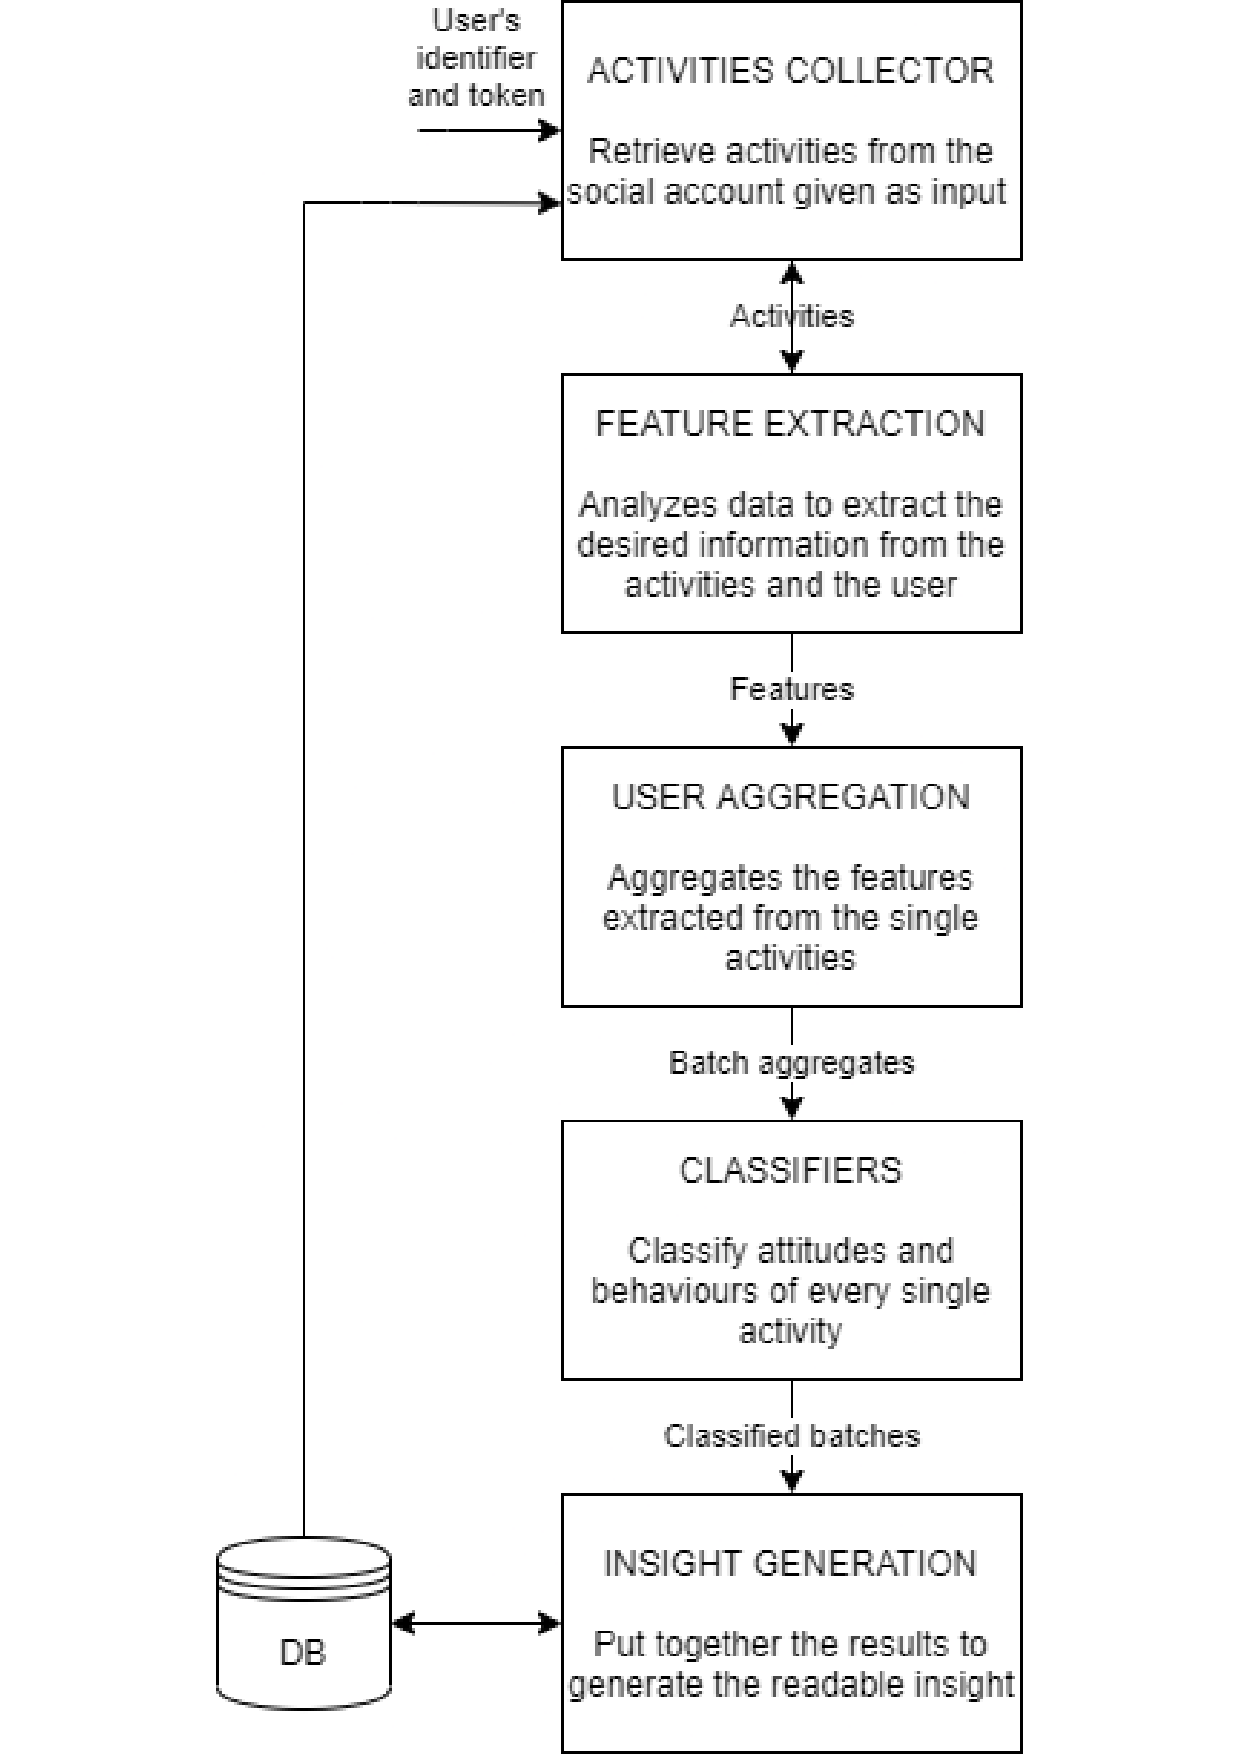
\includegraphics[width=%
    0.95\textwidth,height=10cm,keepaspectratio]{img/components}
    \caption{The architecture components}
    \label{fig:components}
\end{figure}

In this section, the architecture is decomposed into its components. Each component works on the input of the previous one to carry out a step of the whole process described previously.
Totally, 5 components have been identified: activities collector, features extractor, user aggregator, classifiers and the insight generator. They are shown in Figure~\ref{fig:components}:


Next, the logic of each component is provided, illustrating what each one does, its input, and output.

\subsection{Activities collector}
This part deals with the downloaded of user's content from social networks through the services offered by the public APIs of each platform.
The data includes information about the user, such as social name, number of followers and friends, location, and then her activities.
An activity is usually characterised by some text, optional attachments such as media or files, a creation date, the number of likes, shares and comments, and, sometimes, information derived from the geolocation.

This component takes as input a list of IDs, one for each social network connected to the user, that identify all her profiles. Some social media, like Facebook and Instagram, also require an access token necessary, together with the user ID, to consult, through the API, the content of that profile.
These tokens are released directly at the organization that is handling the user authorization.

For each social network, the system need to know at which point the data has been previously downloaded. Usually, the IDs identifying the posts are ordered and the API allows you to specify the point the download should start from using an ID.
As output, the components returns a social profile composed by significant user's information and the list of new activities. With new, it is meant all the content that was not previously downloaded by past requests.
Finally, the last activity of the timeline is used to update the point the data has been fetched.

The collector interacts with many different social networks. To do it, this service should run in a dedicated process and the communications with each platform should be parallelized.
This is necessary because many socials provide free API plans which limit the number of requests in a given time window. So, in case one of the limits is reached, it should not cause a critical bottleneck that freezes the whole system.

\begin{multicols}{2}
\begin{verbatim}
//input
[
    {
        "socialID": 1234,
        "userID": 8564
    }
]

//output
[
    {
        "postID": 123456,
        "socialID": 1234
    }
]
\end{verbatim}
\end{multicols}

\subsection{features extractor}
This component works on the downloaded content to extract significant features for the following step.
From the previous part it receives data both about the user's information and about her activities. While the first one is quite structured and does not need deep analyses, the activities carry raw texts and images which have to be processed to extract the desired information.
First of all, the text of each activity is observed and analysed to extract significant features for the classification models, in particular for the psychological ones.
A standard \emph{Natural Language Processing NPL} library is used. It allows to observe some superficial characteristics such as the number of sentences, words, characters, capital letters and the use of punctuation.
Then, giving the environment we are working with, that of social media, it is important to handle properly hashtags, external links and emojis.
The first two, as well as any mention or @tag, are usually returned by the social network's API. So, it is not necessary to extract them from the raw text.
On the other hand, emojis are treated like any other character by the API. Therefore, they need to be parsed carefully.
Taking care of emojis is extremely important because on social media they are abused by the majority of users and, thanks to their variety and intuitiveness, they can reveal a lot about the traits of a person.



\clearpage
\newpage

\chapter{Implementation}
This chapter describes the implementation of a prototype of the system.
It shows how each component was implemented to deal with the requests' limits of external services.
Then, the interaction between them is explained showing the data flow starting with the user request to the final response.
Finally, the techniques used for each classifier are introduced.

\section{Components interactions}
Generally, the system is composed by a main request which mobilizes the download of a user's profiles, their analysis and finally their classification.
This process ends with a series of classified batches, of monthly time duration, that are stored in the database.
Then, the call to obtain the final results starts the insight generator shown in Section~\ref{sec:Generator} which merges together the partial results and return the final insight at the user level.

These different types of requests are handled by the request handler which is represented by the user's endpoint, the only interface to the outside of the system.
As said before, it also allows to add and modify the system's users.
The download request is the one that requires communication between multiple components.

This prototype allows the interaction and the download of social profiles only from Twitter.
Indeed, while data from Twitter are publicly accessible through its APIs, other social media, such as Facebook and Instagram, require an access token for each consulted user.
To obtain the access token, a demo video that shows what the system does must be provided, the data treatment has to be described precisely, and each person should accept to share its data.
\subsection{Download Request}
The endpoint /newactivities represents the most complex one that involved the majority of the components.
In this prototype, the components execute synchronously. In the moment the request is received, the activities collector is executed and the system waits for it to end and return its results.
Then, all the downloaded activities are analysed. Once all the features are extracted, they are divided in batches and finally classified and stored.

The process starts with the ID of a user which is used to search on the database the Twitter ID associated with that specific user. 
This is used by the activities collector to download the new content. As said before, the system is structured to download only new activities and not the whole timeline.
To do it, it is used the ID of the oldest activity of the second-to-last stored batch because the last one could contain only a part of the content posted in a month. 
The drawback of this choice is that activities already contained in the last batches are downloaded and classified again but it is necessary to ensure a full download. Moreover, a maximum of thirty days is downloaded twice which is a limited number compared to the whole user's timeline.
The collector uses \textit{Tweepy}, a Python library, to access the Twitter API. It allows to download a user's content specifying its ID and the point from where the download of its activities should start.
Once the download is complete, an object \textbf{User} is created. It contains both social information about the profile, such as creation date and description, and the list of all the fetched activities. Each one is represented by a \textbf{Post} object that contains everything about the downloaded content: creation date, number of likes and retweets, its text, list of media, hashtags and urls.
The user object is passed to the next component, the analyser, with a standard class method call by the request handler.

The analyser is the component that extracts, starting from the single activities, the significant features.
Considering the various classifiers implemented, different types of features are extracted.

First of all, the information contained into the fetched tweet object that does not require any processing or further analysis is kept also in the analysed Post. This includes its id, the creation date, the number of favourites and retweets, the language of the tweet, and its type.
There are 4 different types of tweets: original, reply, retweet, and quote.

The text component of the post is used to obtain fundamental textual features. This analysis is carried out using \textit{SpaCy}, an open-source Python library for natural language processing.
Before executing the Spacy pipeline, some pre-processing is done. Whitespaces are normalized, multiple spaces and new lines are treated as a single space. The number of capital letters is memorized and then the text is converted completely in small caps.
Then, the text is passed through all the components of the pipeline. It starts with the \textit{tokenizer} which segments text into tokens like words and punctuations marks. The \textit{lemmatizer} is now involved to reduce each word to its canonical form, called \textbf{lemma}. Then, each token is assigned a part-of-speech tag thanks to the \textit{tagger}.
At this point, 2 custom components are added. First, the extension \textit{spacymoji} is used to handle emojis efficiently. Then, the last component handles \#hashtags and @mentions so that the lemma does not contain special symbols \# and @.
The result of this pipeline is a list of tokens that represent the bag of words extracted from the text. Each token contains information such as the raw word, its lemma, and its POS tag.
Now, other more generic features are extracted. spacy allows counting automatically the number of sentences, words, and characters. Starting from this data, many averages are computed such as number of words per sentence and characters per word.
To conclude, the tokens extracted before are divided into three different sets: words, stop words, emojis, and punctuation.
This distinction is important because we that our classification models could treat each set differently.
Stop words refer to the most common words in a language. There is no single general list of stop words and any group of words can be chosen. Spacy provides its own list for each supported language.
The punctuation set includes all the standard punctuation marks but \# and @ that are often special symbols on the social networks.
Finally, the words set contains all the other words.
Each set is memorized as a dictionary {\textbf{key} : \textbf{value}} used as a counter where \textbf{key} is the text of the token and \textbf{value} is its number of occurrences in the tweet.  
Some of the pipeline operations described, such as the lemmatizer, the tagger, and the stop words list, are language-dependent. In this prototype, the Italian module of Spacy has been used so these three specific phases are optimized only for that language. Anyway, Spacy provides plenty languages models and also a multi-language one.

Another important group of features is that describing the content of a tweet. For this purpose, \textit{DandelionAPI}, a semantic analysis service was used. It works on unstructured text to extract its meaning. 
In particular, it offers two important functionalities: entity extraction and sentiment analysis.
The first one can be useful to understand a person's interest and therefore is not used in this prototype which does not implement that specific classifier.
The second one may have an important role with respect to psychological characteristics.
It allows identifying whether an opinion contained in the tweet is negative, neutral, or positive. 
DandelionAPI is accessed with restAPIs and one request is necessary for each piece of text that need to be analysed. Moreover, it supports more than 40 languages, including Italian and English, and it can also compute automatically the language detection of the text given as parameter.
The response is structured in JSON and contains: the detected language, a sentiment score and a sentiment type.
The score is a more precise indicator ranging from -1.0 (totally negative) to 1.0 (absolutely positive) while the type is a descriptive label which can be \textit{negative}, \textit{neutral}, or \textit{positive}. 

Finally, the set of features regarding the media entities is created. Twitter supports three types of media: photos, videos and animated gifs. They are generally treated as \textit{media entity}.
The TwitterAPI returns, for each entity, a exhaustive series of descriptive attributes. Of interest for this prototype are the media type and the media URL.
The first one is important to understand in which way a person ten to communicate while the second one represents an important part of the tweet's content.
They may be analysed in order to detect emotion, entities and, places in a way similar at that done for the text.
So, even though images and videos are not used in this demo, mainly because rarity of free computer vision services, the URLs are downloaded to easily allow future improvements.

Once all the features are extracted, the same \textbf{User} object taken as input is modified replacing the list of \textbf{Post} object with a list of features which represents the analysed tweets.
This new object is passed to the next component, the aggregator.

The aggregator has to goal to divide the posts in batches and then compute the aggregates for each batch.
As introduced before, in this prototype the batches are temporality-based and each one ranges over a period of one month.

\clearpage
\newpage

\chapter{Conclusions}
This dissertation answers to the initial question that regarded both the feasibility of behaviour extraction from social media and the usability of the obtained results in the production environment.
To do it, a system that uses twitter activities to extract nine different characteristics is presented.
It differs from the actual state of the art solutions for many reasons. First of all, it automatizes the analysis of a profile to extract its characteristics and is not limited to analyse a list of given activities.
Then, the system allows the integration of the insights once new activities are posted without the necessity of computing again the whole timeline.
Furthermore, in addition to the general results, there is a classification for each month of activity of a user that allows displaying temporally the results to observe fluctuations and compare different profiles.

The architecture was designed taking into consideration the requirement imposed by the GDPR.
In particular, the principles of data minimisation and data accuracy have been studied and both architectural and implementation choices were done to meet these requirements.

Many different aspects have been classifiers. The ones about the psychological aspects implemented ML solutions while the others, due to the lack of available data, implemented non-ML algorithms.
Concerning the ML solutions, they only support the Italian language since models have been trained only on a dataset of activities completely written in Italian.
The results' performances of the MBTI classifiers are discrete but lower than than the actual state of the art. However, no particular setups for the features have been used. So, there is ample room to improve them. 

Finally, the implemented user dashboard showed how easily the architecture allows monitoring and inferring insight for a person.
The analyses of the profiles carried out in Section~\ref{sec:nonMLIns} proved how the system can be useful in the comparison of profiles in order to understand their differences.

\section{Future work}
Many new aspects that can be added or improved.
Firstly, the system is designed to interact with different social networks. Due to the privacy policies of some of them, the implemented prototype uses only Twitter data.
So, adding some new platforms among the most famous, such as Facebook and Instagram, could be a first interesting improvement.

Then, the performance of the existent classifiers may be improved. Starting with the solution based on ML models, two addition can be done. First of all, multi-languages supports can be added my training new models on the new language we want to add and then by merging the results coming from different languages. Secondly, new features and algorithms should be tested. For example, complex services that extract significant personality info both from text and images could be integrated into the system.
Regarding the other classifications, some of them could be improved by collecting data that can be used to train more accurate models. For example, the influence role classifier could improve significantly by training a model with a dataset of profiles labelled with the corresponding influence class.

Also, new classifiers can be added to the system. There are a lot of useful aspects and behaviours which a company could take advantage from. For example, being able to extract someone's interests from her online activities would improve significantly the use cases of the system here proposed.
During the realization of this thesis, an approach to extract user's interest from text and images using Wikipedia categories was tried. It was presented by Christian Torrero from \textit{U-Hopper} here \cite{torrero2018wikipedia}.
The implementation of such service has not been completed but could certainly be one of the next steps.

Then, even though the prototype was implemented following the batch-based architecture with very good results, trying and testing the other proposals and setups would certainly prove the qualitative analysis described in Section~\ref{sec:systemArch}.
Also, new setups for the insight generation algorithm introduces in Section~\ref{sec:Generator} should be tried and evaluated.

To conclude, this thesis explored some of the issues related to the extraction of behavioural aspects from social media and their use in the production environment and proposed a system that answered the initial problem with satisfying results.
However, the system is still amendable with what is described in this conclusive section.

\clearpage
\newpage

% Bibliography
\printbibliography[heading=bibintoc, title={References}]
\end{document}
